%%%%%%%%%%%%%%%%%%%%%%%%%%%%%%%%%%%%%%%%%
% Journal Article
% LaTeX Template
% Version 1.4 (15/5/16)
%
% This template has been downloaded from:
% http://www.LaTeXTemplates.com
%
% Original author:
% Frits Wenneker (http://www.howtotex.com) with extensive modifications by
% Vel (vel@LaTeXTemplates.com)
%
% License:
% CC BY-NC-SA 3.0 (http://creativecommons.org/licenses/by-nc-sa/3.0/)
%
%%%%%%%%%%%%%%%%%%%%%%%%%%%%%%%%%%%%%%%%%

%----------------------------------------------------------------------------------------
%	PACKAGES AND OTHER DOCUMENT CONFIGURATIONS
%----------------------------------------------------------------------------------------

\documentclass{article}

\usepackage{blindtext} % Package to generate dummy text throughout this template 

\usepackage{tikz}
\usetikzlibrary{arrows.meta}
\usepackage{adjustbox}

% define style for ``not visible nodes and edges''
\tikzset{bled/.style={black!40, line width=1pt, fill=white}}

\usepackage{graphicx}



\usepackage[english]{babel} % Language hyphenation and typographical rules




\usepackage{hyperref} % For hyperlinks in the PDF

\title{Understandable Bayesian Recommendation Engine - user guide}
%\author{Martin Molan \\
%	Jozef Stefan International Postgraduate School  \\
%	\and 
%	T \\
%	His Company / University \\
%	}

% Hint: \title{what ever}, \author{who care} and \date{when ever} could stand 
% before or after the \begin{document} command 
% BUT the \maketitle command MUST come AFTER the \begin{document} command! 





\begin{document}

% Print the title
\maketitle

%----------------------------------------------------------------------------------------
%	ARTICLE CONTENTS
%----------------------------------------------------------------------------------------
 

\section{From classification to recommendation}
In order to construct a recommendation engine we first start with a classifier. Our basic task is to predict if the material will be usable for a blind student. Instead of predicting just the usability (1 or 0) we can predict the \emph{probability} for the material to be usable (\emph{probability for class 1}). We then rank materials according to their probability to be useful. Effectively we rephrase the question of which material is the most suitable into which material is the most \emph{likely} to be suitable. 
\bigbreak
So in order to construct a \emph{predictor} we first have to construct a \emph{classifier}. How does this classification take place? The documents characteristics determine which features are relevant.Than we see the user preferences for those features; if the preferences are mostly negative the resource is classified as un-accessible. Otherwise the resource is classified as accessible.
\bigbreak
So in order to understand the student we just have to understand his/her preferences expressed as weights right? Not entirely - we give the estimates for parameters even if we now very little about the student. So it is also useful to understand how \emph{certain} we are in our estimate. This is where Gaussians come into play.


\section{Why should I care about the Gaussians?}
Simply - they give you much more information than a number. Standard algorithms give their estimate for parameter. We give you a range where we believe the parameter to be. And of course, our range changes the more information about the learner we get. 
\bigbreak
The more we know about the preferences of the user, the tighter our range estimate becomes. How can you see that on the graph? Just check the 'width' of the hill. \emph{The wider the hill the more uncertain about the parameter estimate we are}. The narrower the hill the more certain we are - if the hill deforms into a single line than we are absolutely certain in our estimate. But we will need a lot of data before we are that certain. Also we don't stay that certain till the end of time - over time we slowly loose certainty - our hills become wider. On the figure \ref{f:g}, we can see that we care much more certain into blue parameter than into orange one. Again the only thing that communicates certainty is is the shape. 
 

\begin{figure}[h!]
\centering
\caption{Two Gaussian. Can you guess which parameter we can estimate with more certainty?}
\label{f:g}
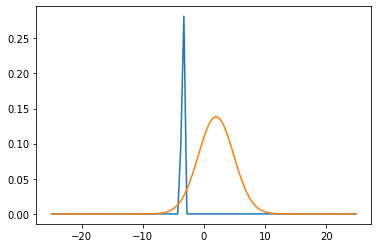
\includegraphics[width=8cm]{two_gauss}
\end{figure}

\end{document}
